\documentclass[english]{article}

\usepackage{graphicx}
\usepackage{grffile}
\usepackage[T1]{fontenc}
\usepackage{babel}
\usepackage{wrapfig}
\usepackage{hyperref}

\date{\today}

\graphicspath{{Pictures/}}
\begin{document}	
	\begin{titlepage}
		\pagenumbering{gobble}
		\begin{figure}[!t]
			
\includegraphics[width=\linewidth]{up_logo.png}
		\end{figure}
		\vspace*{\stretch{1.0}}
		\begin{center}
			\huge{Project: Mind Mapped PIM}\\
			\large{Client: IMINSYS}\\
			\vspace{10mm}
			\huge{Team: A-Cube-N}\\
		\end{center}
		\begin{center}
			\begin{tabular}{ c c c }
				Dunkley, Nathan & Grobler, Arno & Lochner, Amy \\
				\texttt{14145759} & \texttt{14011396} & \texttt{14038600}\\
				& Maree, Armand &\\
				& \texttt{12017800} &
			\end{tabular}
		\end{center}
		\begin{center}
			Department of Computer Science, University of Pretoria
		\end{center}
		\begin{center}
			\today
			\begin{figure}[!h]
				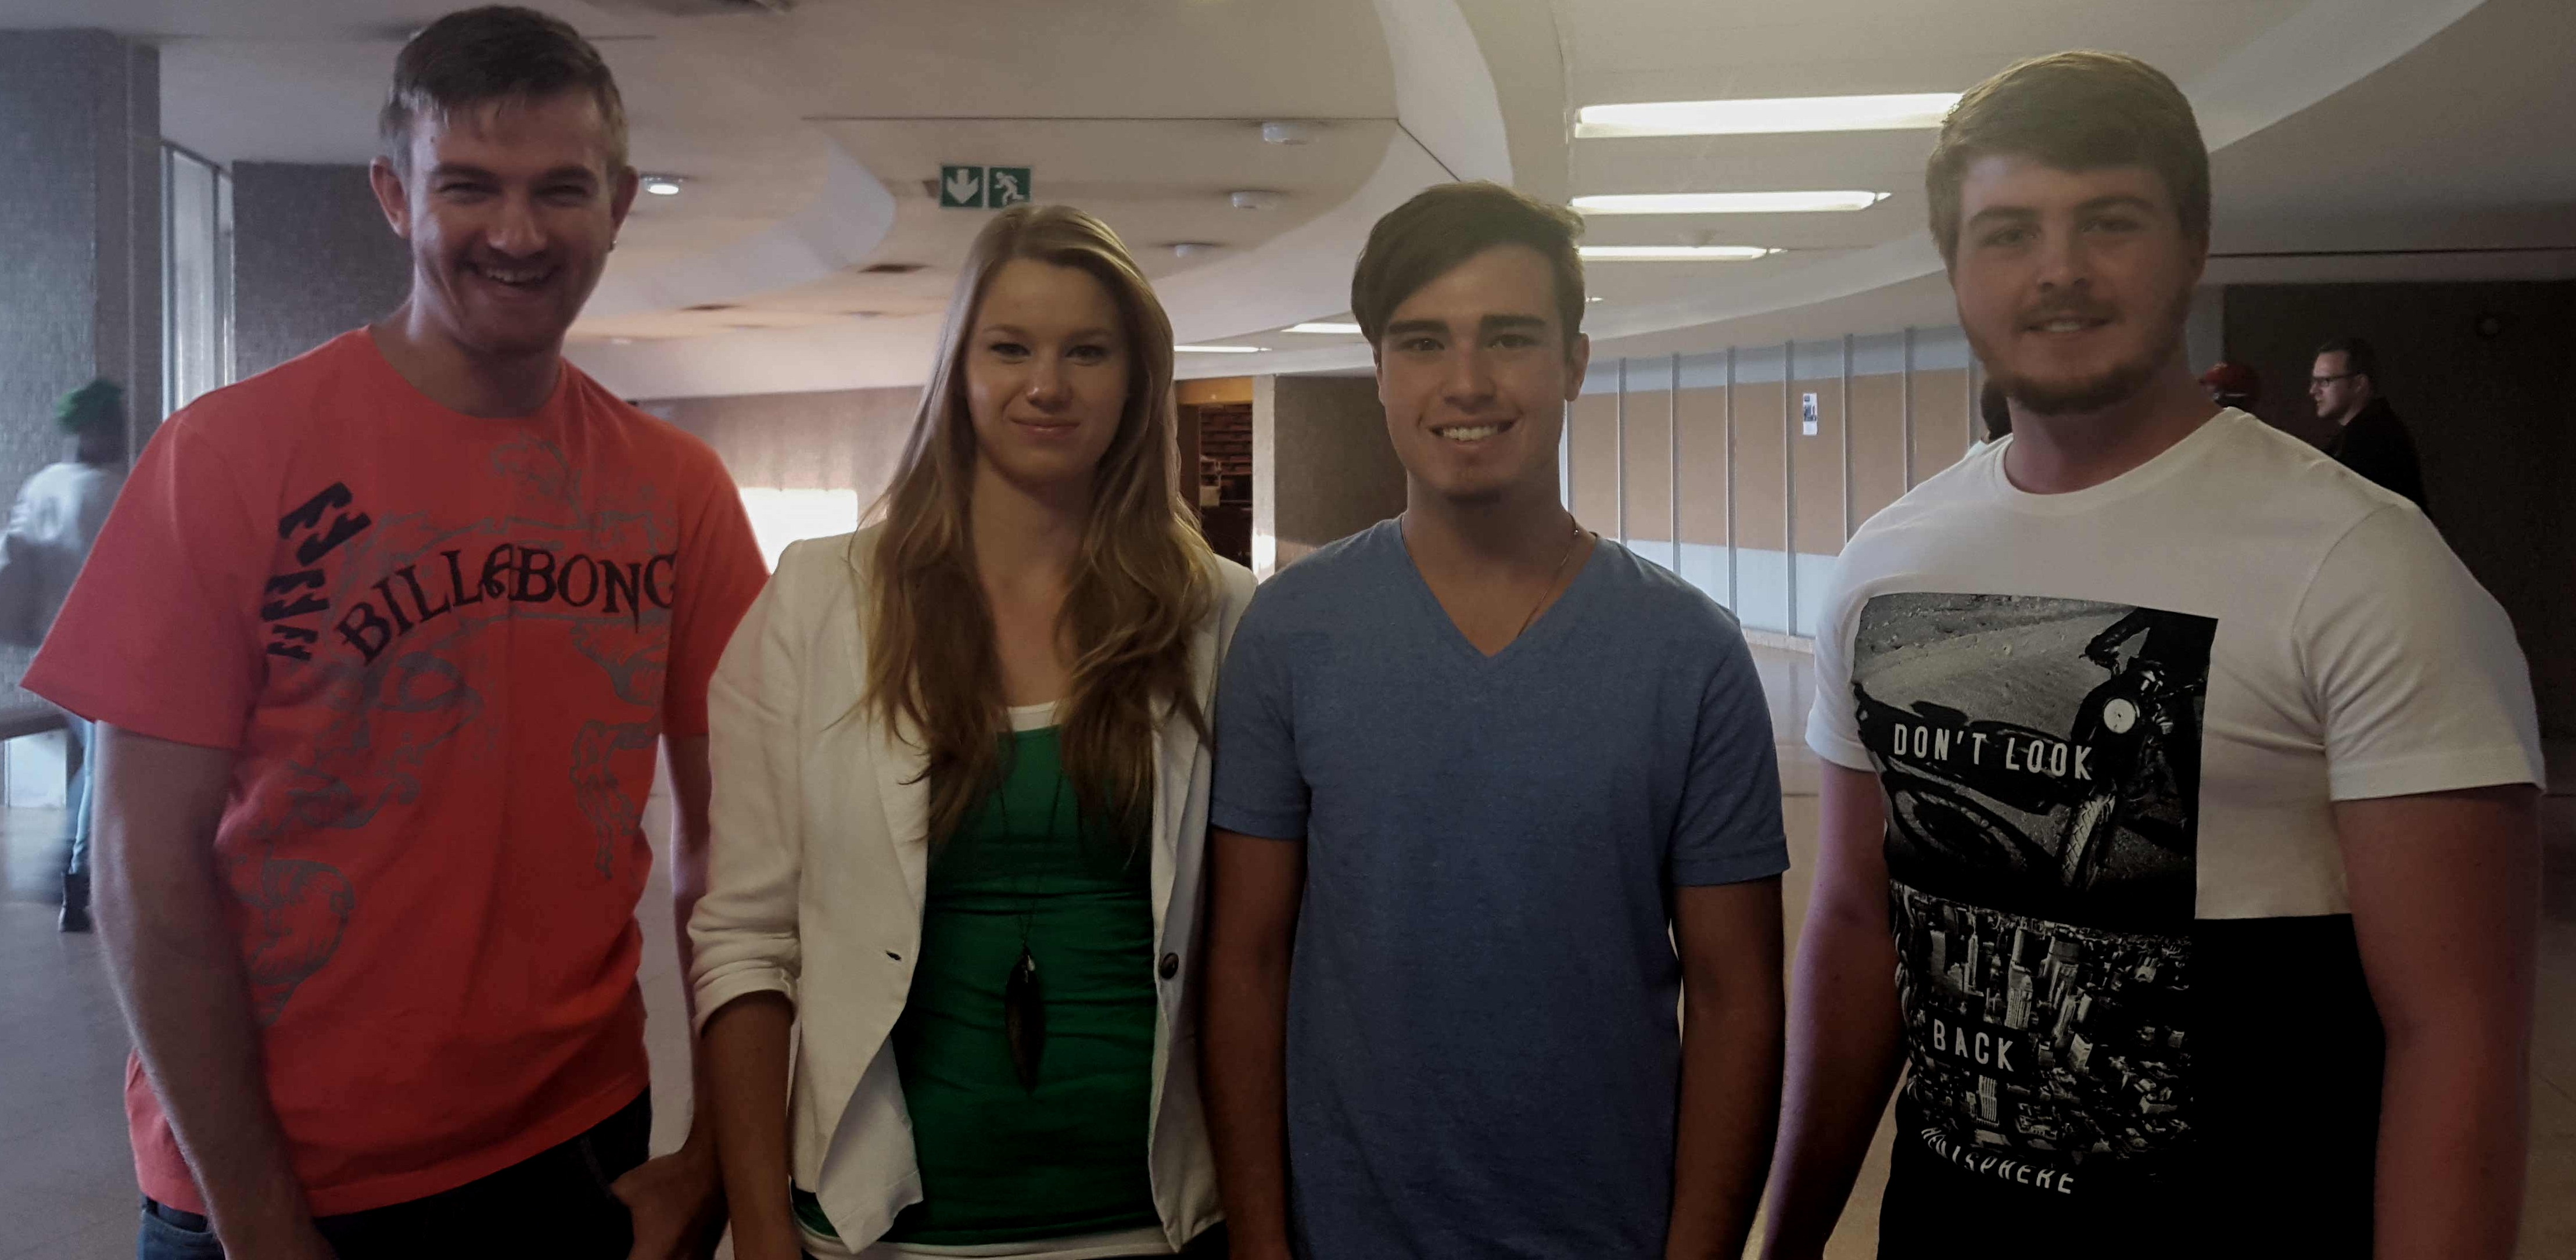
\includegraphics[width=\linewidth]{team.jpg}
			\end{figure}
		\end{center}
		\vspace*{\stretch{2.0}}
	\end{titlepage}
	\newpage
	\tableofcontents
	\newpage
	\pagenumbering{arabic}
	\section{The Team}
		\subsection{Nathan Dunkley}
		\begin{wrapfigure}{l}{5cm}
			\begin{center}
				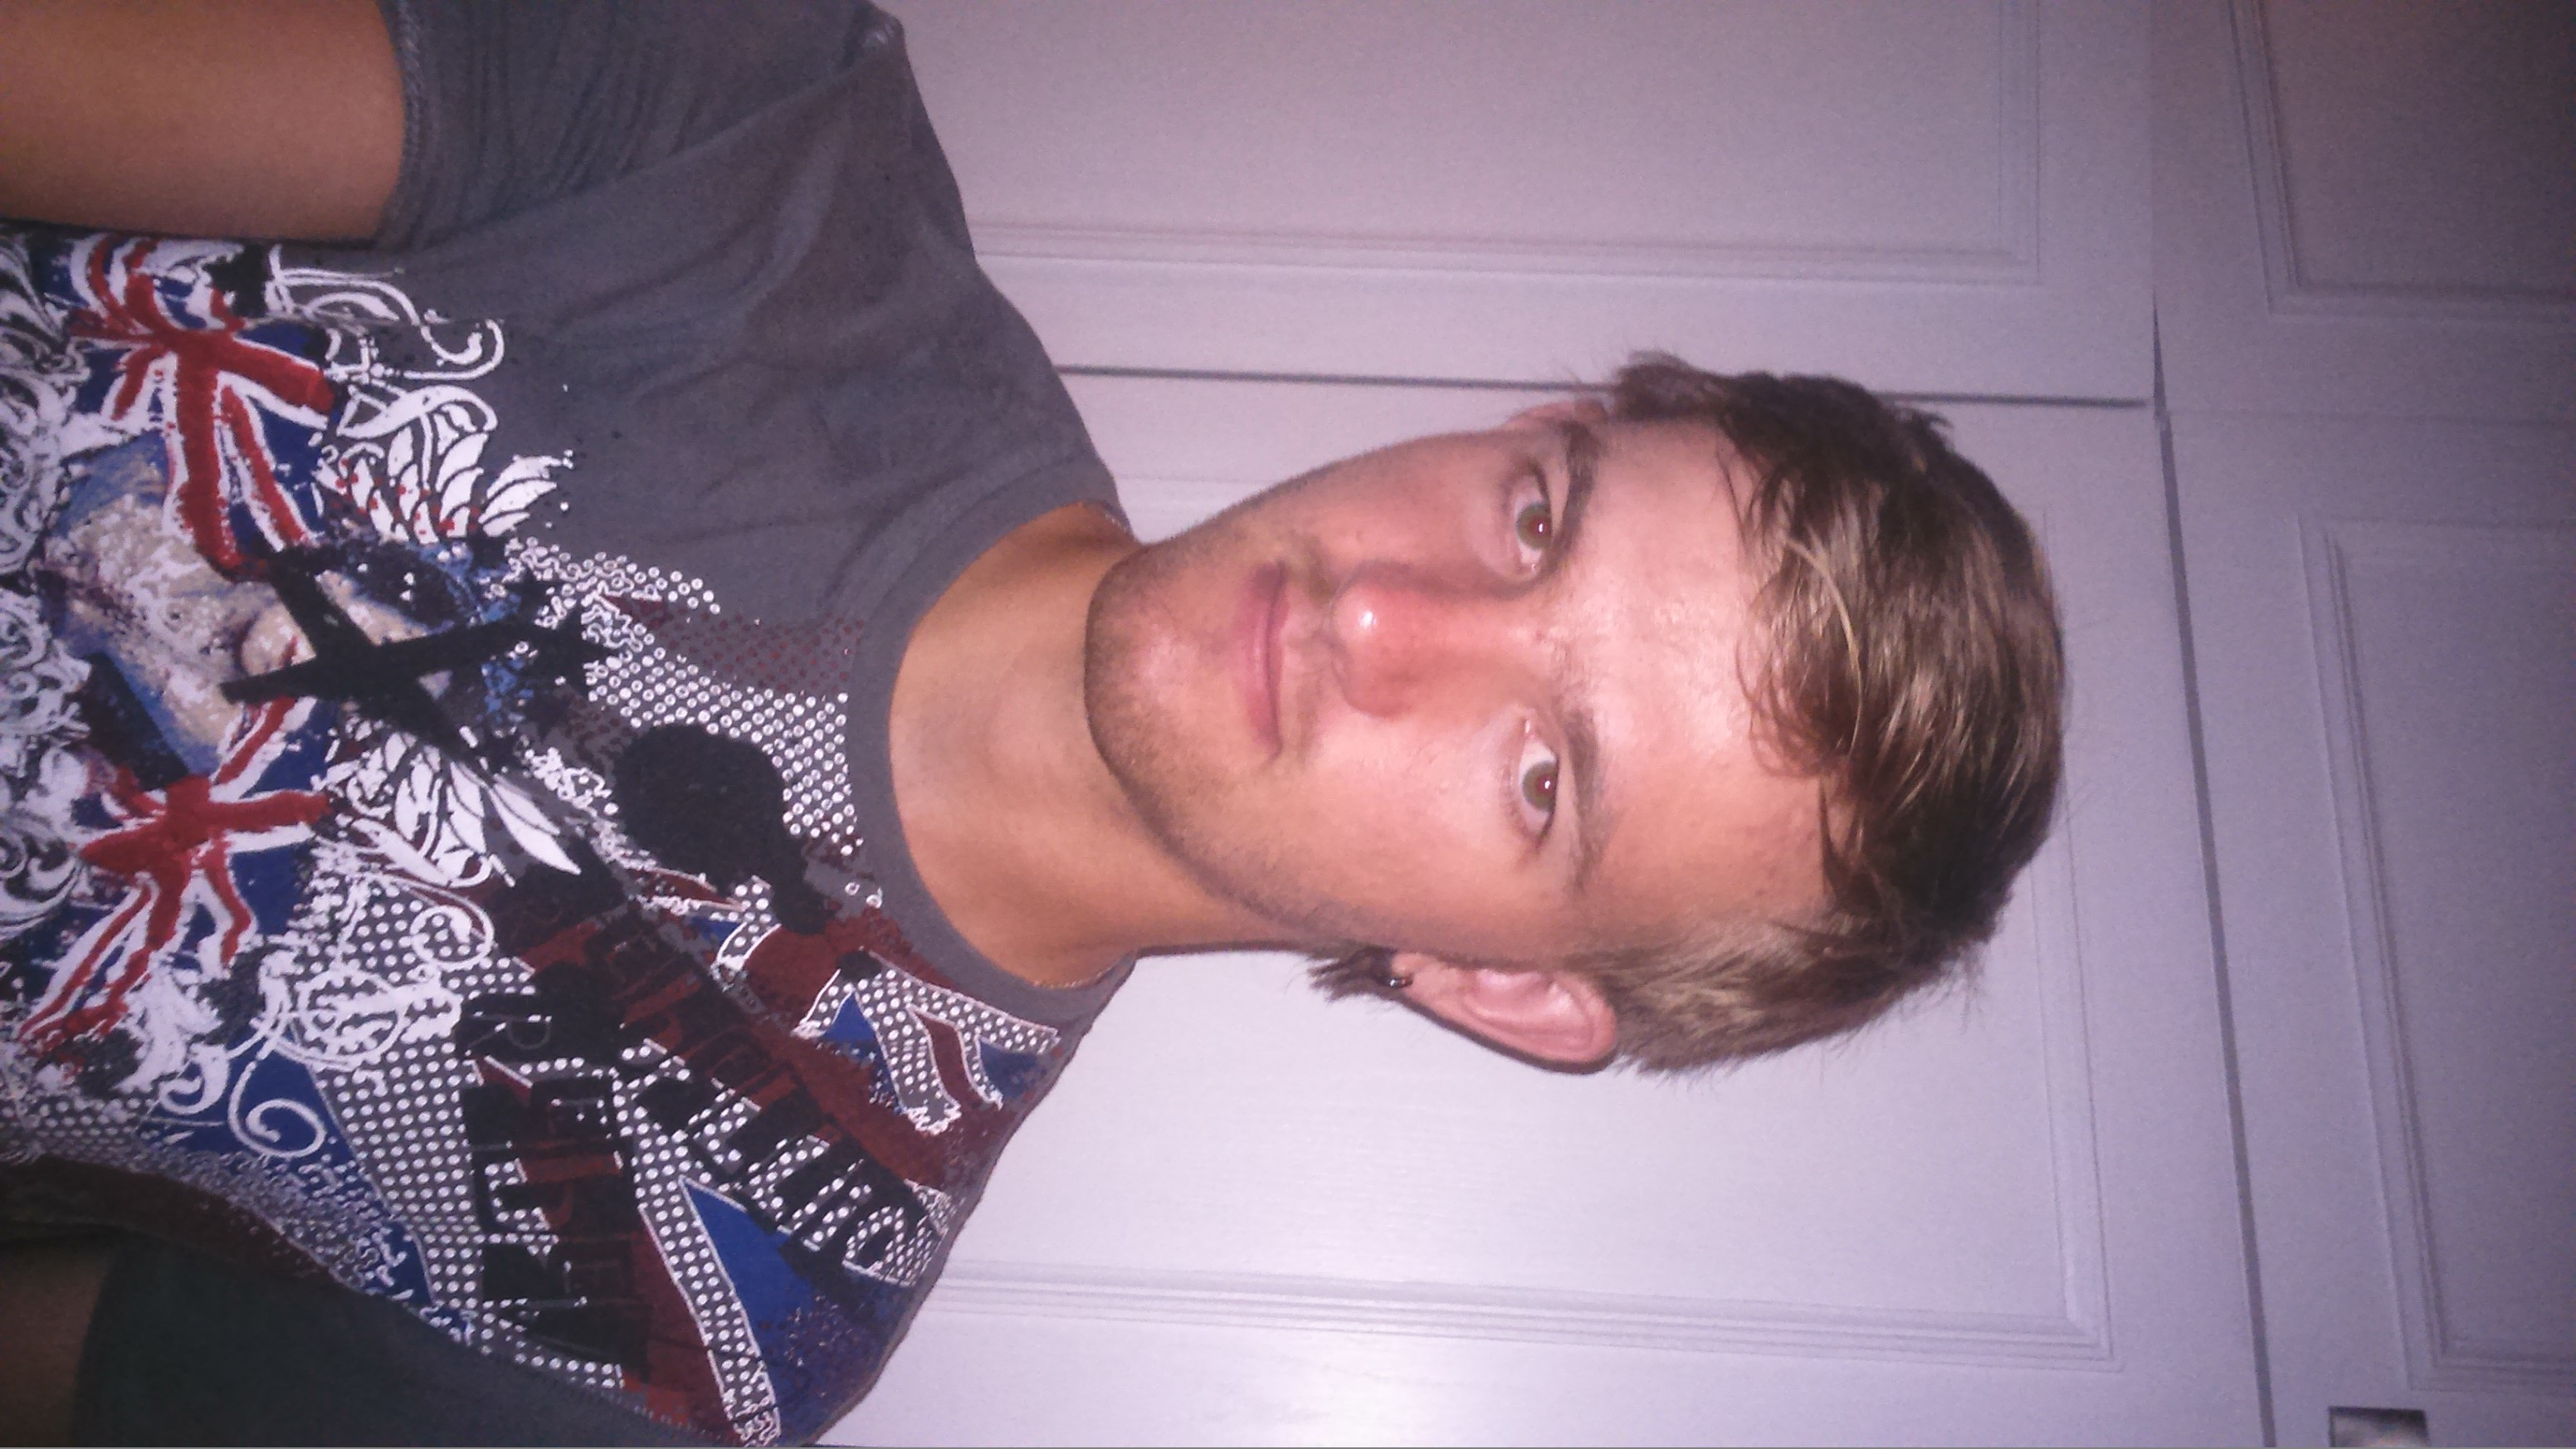
\includegraphics[width=8cm, height=4.5cm, angle=90]{nathan.jpg}
			\end{center}
			\end{wrapfigure}
			\paragraph{Interests and Hobbies}
			My interests include playing and watching sport, specifically motorsport (Formula One, World Endurance Championship), cricket, tennis and golf. I play tennis twice a week at a club. I also like to listen to music and read books as well as play games on PC.
	
			\paragraph{Technical Skills}
			I'm more of a follower than a leader and I'm good at getting on with work once the tasks have been delegated to the members of the group. I enjoy working on tasks that interest me and don't mind working long hours to get it done, once I've put my mind to it. I have some experience in multiple programming languages and I enjoy learning new skills when I can. I also enjoy solving problems.
	
			\paragraph{Past Experience}
			Minor experience in Android Development.
	
			\paragraph{Non-Technical Strengths}
			\begin{itemize}
				\setlength\itemsep{0.2em}
				\item Fast Learner
				\item Willing to Learn
				\item Flexible
			\end{itemize}
	
			\paragraph{Motivation}
			To do..
		
		\newpage
		\subsection{Arno Grobler}
			\begin{wrapfigure}{l}{5.1cm}
				\begin{center}
					
\includegraphics[width=5cm]{arno.jpg}
				\end{center}
			\end{wrapfigure}
			\paragraph{Interests and Hobbies}
			My interests include collecting music, long distance running, painting and drawing, reading, computer games and obviously spending most of my days programming. Not only do I want to program as a profession, it is also a hobby for me. Integrating my other hobbies into my programming is my passion.
			
			\paragraph{Technical Skills}
            I pride myself in always looking for new skills and for me, learning a new technical skill is the best part of the experience. I enjoy making my projects look visually pleasing and spend as much time making a working, functional program as I do making it look good. I have good logical and problem solving skills and enjoy problems presented to me in computer science. My technical skills stem from Mathematics and computer science, especially those skills from data structures and algorithms and programming logic.
			
			\paragraph{Past Experience}
            I have created static websites for companies before, my most recent one is (\href{http://bodytalkbethlehem.com/}{http://bodytalkbethlehem.com/}) and (\href{http://honeydewpools.co.nf/}{http://honeydewpools.co.nf/}).
			
			\paragraph{Non-Technical Strengths}
			\begin{itemize}
				\setlength\itemsep{0.2em}
		       	\item Eager learner
		       	\item Organised 
		       	\item Good time management
		       	\item Good communication skills
		       	\item Creative
			\end{itemize}
			
			\paragraph{Motivation}
			To do..
		
		\newpage
		\subsection{Amy Lochner}
		    \begin{wrapfigure}{l}{5cm}
				\begin{center}
					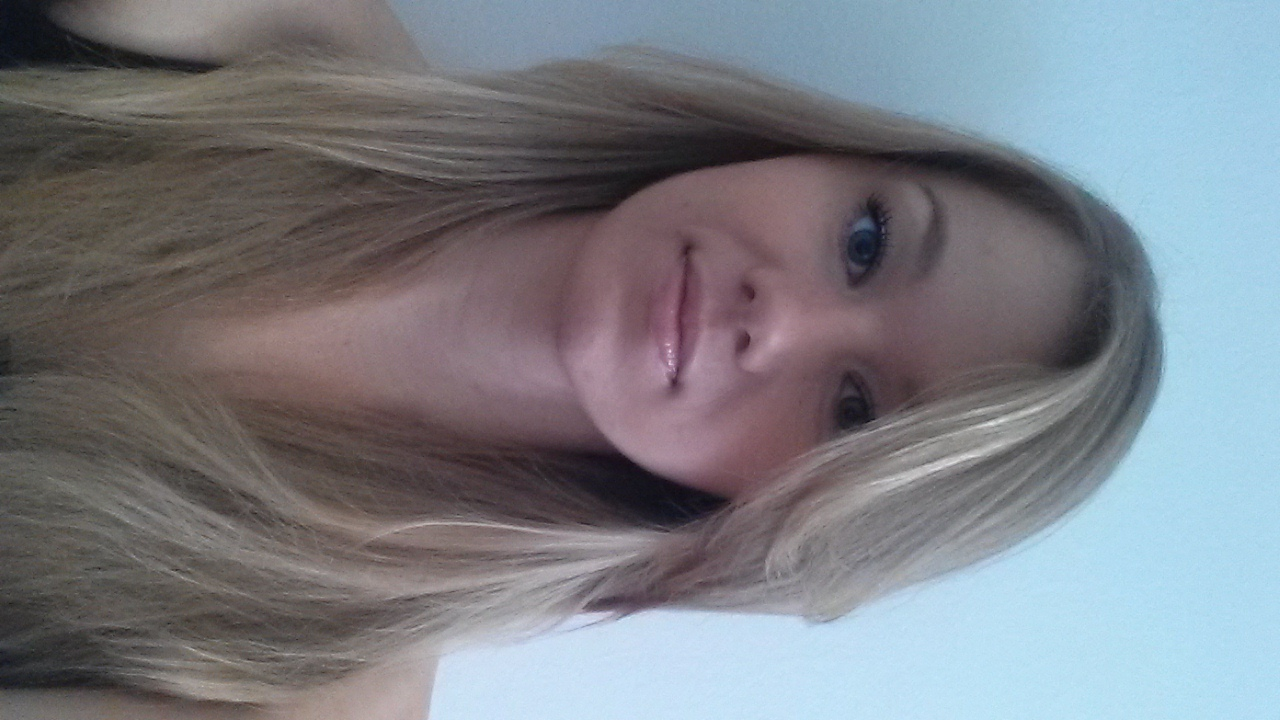
\includegraphics[width=8cm, height=4.5cm, angle=90]{amy.jpg}
				\end{center}
			\end{wrapfigure}
			\paragraph{Interests and Hobbies}
			My interests include music, classic cars, cooking, traveling, breeding Shetland sheepdogs. My hobbies include reading, playing piano, camping, 4x4ing, tennis, training my dog, mountain biking and horse riding.
			
			\paragraph{Technical Skills}
			I am good at determining functional requirements of a system. I can place myself in the users shoes, this is valuable when determining how the user will intend to use a system. I can follow business logic easily and I have experience in databasing, Informatics, Statistics, Mathematics, multiple programming languages and Human Computer Interaction.
			
			\paragraph{Past Experience}
			I have built a fully functional, responsive website. I have helped a company modify their website. I have also observed (by job shadowing) the process of creating a system for a business and have noticed which qualities have caused them to excel and which have caused them to fail. I intend to use that knowledge to keep our team constantly progressing forward.
			
			\paragraph{Non-Technical Strengths}
			\begin{itemize}
				\setlength\itemsep{0.2em}
			        \item Organized
			        \item Good at prioritising 
			        \item Team player
			        \item Good leader
			        \item Optimistic
			        \item Quick learner
			        \item Determined
			\end{itemize}
			
			\paragraph{Motivation}
			I would like to do this project because I think it is a very creative idea and poses a challenge. It will be interesting to combine a number of different technologies and develop a means by which to sort through and process data while keeping the personal information secure. It will test our abilities, make use of our strengths and give us an incredible learning curve.
		
		\newpage
		\subsection{Armand Maree}
			\begin{wrapfigure}{l}{5.1cm}
				\begin{center}
					
\includegraphics[width=5cm]{armand.jpg}
				\end{center}
			\end{wrapfigure}
			\paragraph{Interests and Hobbies}
			During my off time I like to socialize with friends and enjoy watching sports. I also like solving puzzles to keep my brain active during holidays.\\
			Tutoring scholars and university students has become a passion for me. I always look forward to these sessions.
			
			\paragraph{Technical Skills}
			I am good at solving complex problems and building data structures. I believe this is a valuable skill to complete any project, especially in the field of computer science.
			
			\paragraph{Past Experience}
			I have developed websites for other start up companies and I also have a website of my own (\href{http://www.codehaven.co.za}{www.codehaven.co.za}).
			I also have some Android developing experience I gained from side projects.
			
			\paragraph{Non-Technical Strengths}
			\begin{itemize}
				\setlength\itemsep{0.2em}
				\item Good leader
				\item Fast learner
				\item Team player
				\item Good communicator
				\item Passionate
				\item Problem solver
			\end{itemize}
			
			\paragraph{Motivation}
			THIS SECTION IS PROJECT SPECIFIC
			
	\newpage
	\section{Project Execution}
		\subsection{Development Methodology}
			\paragraph\indent
			We are planning on using the Agile iterative software development methodology. The reason we have chosen this methodology can be described through the benefits of this methodology:
			\begin{itemize}
				\setlength\itemsep{0.2em}
				\item High degree of collaboration between the client and project team
				\item Allows clients to be involved throughout the project - this requires clients to understand that the work they will see is a 'work in progress'
				\item By using the idea of Sprints new features are delivered quickly and frequently
				\item Focusing on users needs results in each feature incrementally delivering value not only an IT component
				\item The breaking down of the projects into units allows the team to focus of high-quality development, testing and collaboration. Quality is improved by finding and fixing bugs quickly, and realising expectation mismatched quickly
			\end{itemize}
			
			more information on the benefits of this methodology can be found at: \sloppy\url{http://www.seguetech.com/blog/2013/04/12/8-benefits-of-agile-software-development}
			This methodology will allow us to frequently display working progress of the desired system to the client. It will also allow us to have larger, but still manageable, portions of the work done between each meeting. We believe this is essential in order to make faster progress while still being able to make changes to the system should the requirements change. See figure \ref{fig:developmentMethodologies}.
			
			\begin{figure}[!h]
				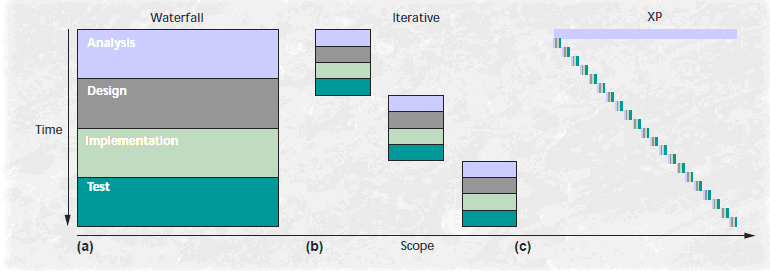
\includegraphics[width=\linewidth]{developmentMethodologies.png}
				\caption{Waterfall vs Iterative vs Extreme Programming methodologies.}
				\label{fig:developmentMethodologies}
			\end{figure}
		
		\subsection{Client Updates}
			\paragraph\indent
			 We will keep the client informed on our progress via frequent face-to-face meetings in order for IMINSYS and developers (students) to discuss important milestones in the project, should it be necessary. Regularly updates (weekly or fortnightly) can be made known to the client via email or via face-to-face meetings. We could make use of a tasking system in which we set a number of tasks we wish to achieve and make this available to the client in order for them to monitor our progress.
			
		\subsection{Initial Ideas}
			\paragraph\indent
		
		\subsection{Potential Technologies}
			\paragraph\indent
			\begin{itemize}
        		\item   Git and GitHub: A distrabutive version control system that is easy to use and free. It will be used to store and control the code written for the project and thus all code written by group memebers will be easily managed. (http://github.com/). 
    		        \item PostgreSQL: Since we need to have a data store, we could use a PostgreSQL database to store the data.It is a free, open-source, cross-platform, object-orientated database management system. (http://www.postgresql.org/about/). An added benefit is the fact that it has an unlimited database size unlike many other similar technologies.
    		        \item HTTPS: This technology is almost a must as it will increase the systems security by adding needed encryption.
    		        \item Bootstrap: This technology is a powerful mobile first front-end framework for faster and easier web development. It will standardize the way content is displayed for the web front end.
    		        \item IMAP: Something that is integral, is the protocol needed to send emails and read emails such as details or data of user's inboxes.
    		        \item JavaScript/JQuery: Used for client side functionality for example verification of user data.
    		        \item Glassfish Server:  Reference implementation of Java EE and as such supports EJB, JPA, JavaServer Faces, JMS, RMI, JavaServer Pages, servlets, etc. 
    		        \item  JUnit Testing: A unit testing framework for the Java programming language.
    		        \item ART and Dalvik: Android runtime (ART), is needed to compile android source code and run byte code generated from Dalvik.
    		        \item HTML 5 Canvas: used to render information into a visual representation to the user. It is fast and highly scalable
    		 \end{itemize}   
		
		\subsection{Deliverables}
			\paragraph\indent
			 On completion of this project, the following deliverables will be presented to the client
		    \begin{itemize}
		        \item all source code
		        \item all build fields
		        \item a requirements specification document
		        \item a project plan
		        \item architectural design
		        \item test plan
		        \item a user manual
		        \item documentation of all code
		    \end{itemize}
\end{document}
